\documentclass[a4paper]{article}

\usepackage[english]{babel}
\usepackage[utf8]{inputenc}
\usepackage{amsmath}
\usepackage{graphicx}
\usepackage{listings}
\usepackage[colorinlistoftodos]{todonotes}
\title{Emergent Architecture Design}
\usepackage{authblk}

\author[1]{Boudewijn van Groos}
\author[2]{Chris Langhout}
\author[3]{Jens Langerak}
\author[4]{Paul van Wijk}
\author[5]{Louis Gosschalk}

\affil[1]{bvangroos \\
4229843}
\affil[2]{clanghout \\
4281705}
\affil[3]{jlangerak \\
4317327}
\affil[4]{pjvanwijk \\
4285034}
\affil[5]{lgosschalk \\
4214528}

\date{\today}

\begin{document}
\maketitle
\tableofcontents
\newpage

\section{Introduction}
\subsection{Design goals}
\begin{itemize}
    \item Modularity:
    The program can be split into a number of modules. These modules should be
    implemented independently of the other modules. Interaction between modules
    is only possible by making use of defined interfaces.
    \item Continuous Integration: There should be always a working product. Each
    sprint should add one or more feathers.
\end{itemize}

\section{Software architecture views}
\subsection{Subsystem decomposition}

% \begin{figure}[h]
% 	\centering
%    	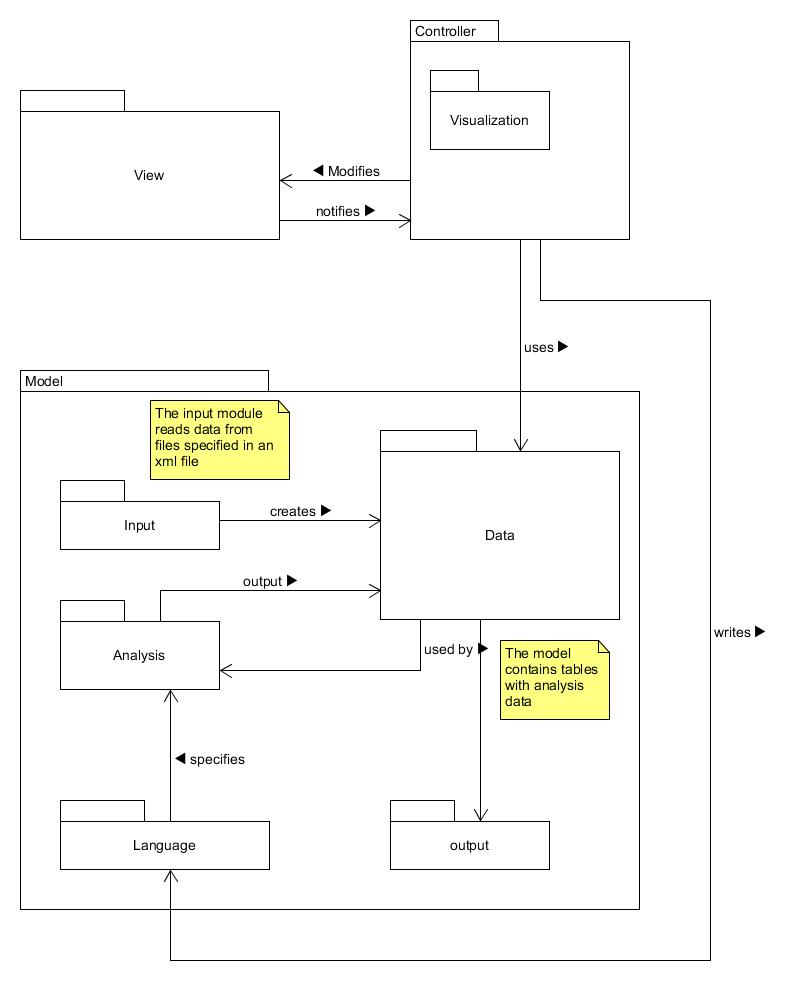
\includegraphics[scale=0.6]{images/modules.jpg}
%     \caption{Modules of the system}
%     \label{fig:modules}
% \end{figure}
The input module should be able to read the data. With that data a dataModel
can be constructed. \\
The Analysis Specification module processes the script that defines how the
data should be analyzed. The user provides this script. This module translate
the script in operations that can be performed by the Analysis Module.\\
The Analysis Module perform the analyses over the dataModel. The output of this
module is the result of the analysis, this is a dataModel.\\
The Visualization module creates a certain visual representation of a
dataModel. For example it can create a box-plot of the creatine levels.

\section{Software architecture}

\subsection{Programming languages and auxiliary programs}
The software will mainly be written in Java since this was obligatory in
the project. For the graphical user interface we make use of the JavaFX
framework and is written using fxml. We use Eclipse and IntelliJ IDEA as IDE to
write the Java code with. For continuous integration and version control we use
Git and Github. 

\subsection{Used libraries}
% JavaFX
% javax.xml
% org.w3c.dom
% Mockito
% apache poi for excell files

\section{Design goals}

\subsection{Availability}

\subsection{Manageability}

\subsection{Performance}

\subsection{Reliability}

\subsection{Scalability}

\subsection{Securability}

\section{Static Analysis}

\subsection{Code quality}
In the project we strive to have good code readability and the code must be easy
to understand. This is also an important part of the static analysis. For
continuous integration we handle the pull based system on Github. For each new
feature that will be implemented the author of that feature must create a new
branch and do all his work in that branch. The master branch must always consist
of a working version of the software. If someone wants to commit he has to
make a pull request. His code will then be reviewed by at least 2
teammembers and eventually fixed before it can be merged with the working
version in the master branch.

\subsection{Checkstyle}
To improve code quality we have code conventions the writer should follow before
his code is accepted. This is done by the Checkstyle plugin in the IDE that makes
sure these conventions are followed.

\section{Functional Tests}


\subsection{Unit testing}
To make sure that all the code works as it should the author must always write
unit tests for the code he has written. We make use of the JUnit framework to
write the tests. To verify behaviour of methods we use the Mockito framework to
stub certain object needed by the method.

\subsection{Integration testing}
The software consists of an amount of modules. We must test that the modules
work together correctly.

\section{Non-functional Tests}

\subsection{Functionality}

\subsection{Usability}
We must also test if the software is user-friendly. Even though the users of the
product are already familiar with analysis software, our application should be
easy to learn. It is essential that the user understands the usage of the
scripting language in our application before he/she is able to use it for
analysis. %interaction design

\subsection{Reliability}


\section{Glossarium}

\end{document}
